\documentclass[12pt,fleqn]{article}\usepackage{../../common}
\begin{document}
Sonlu Öğeler Metotu (Finite Elements Method -FEM-) - 2

Fenics kurulumu icin [2].

[1, sf. 267]'deki örneği altta görüyoruz,

\begin{minted}[fontsize=\footnotesize]{python}
import fenics as fe

mesh = fe.RectangleMesh(fe.Point(0, 0), fe.Point(1, 1), 10, 10)

V = fe.FunctionSpace(mesh, 'Lagrange', 1)

u = fe.TrialFunction(V)

v = fe.TestFunction(V)

a = fe.inner(fe.nabla_grad(u), fe.nabla_grad(v)) * fe.dx

f1 = fe.Constant(1.0)

L1 = f1 * v * fe.dx

f2 = fe.Expression("x[0]*x[0] + x[1]*x[1]", degree=2)

L2 = f2 * v * fe.dx

u0 = fe.Constant(0)

def u0_boundary(x, on_boundary):
  return on_boundary

bc = fe.DirichletBC(V, u0, u0_boundary)

A = fe.assemble(a)
b = fe.assemble(L1)
bc.apply(A, b)
\end{minted}

\begin{minted}[fontsize=\footnotesize]{python}
u_sol1 = fe.Function(V)
fe.solve(A, u_sol1.vector(), b)
fe.plot(u_sol1)
plt.savefig('fenics-sol1.png')
\end{minted}

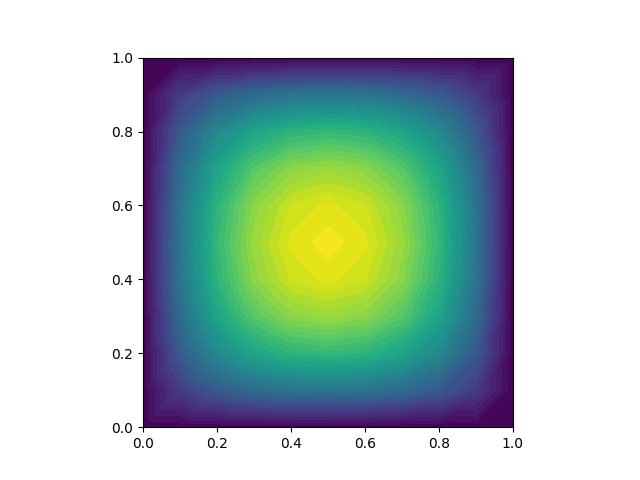
\includegraphics[width=20em]{fenics-sol1.png}

\begin{minted}[fontsize=\footnotesize]{python}
u_sol2 = fe.Function(V)
fe.solve(a == L2, u_sol2, bc)
fe.plot(u_sol2)
plt.savefig('fenics-sol2.png')
\end{minted}

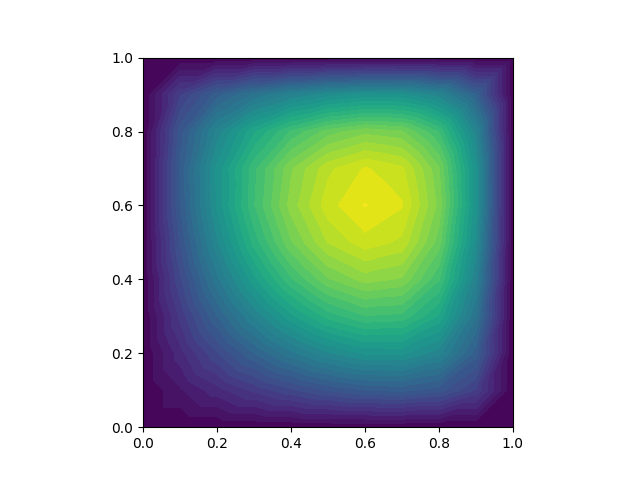
\includegraphics[width=20em]{fenics-sol2.png}



[devam edecek]

Kaynaklar

[1] Johansson, {\em Numerical Python}

[2] Bayramli, {\em Fenics},
    \url{https://burakbayramli.github.io/dersblog/sk/2021/07/fenics-sonlu-ogeler-finite-elements.html}

\end{document}
